\section{Diagrammi - Framework}

Nei digrammi \ref{fig:alt_framework} e \ref{fig:seq_framework} sono rappresentate le interazioni che avvengono generalmente e ad alto
livello tra le componenti del framework, model, view e controller. I segnali inviati dall’utente
vengono ricevuti dalla view, la quale li invia al controller; questo quindi individua l’elemento
funzionale incaricato di elaborare le informazioni e quindi gli inoltra i dati. L’elemento funzionale
del model compie le operazioni richieste e ritorna una risposta o un segnale di conferma. La risposta (o segnale) ricevuto dal controller viene quindi rispedita alla view, che mostrerà all’utente l’esito della sua richiesta ed eventuali informazioni ricevute.

\begin{figure}[H]
	\centering
	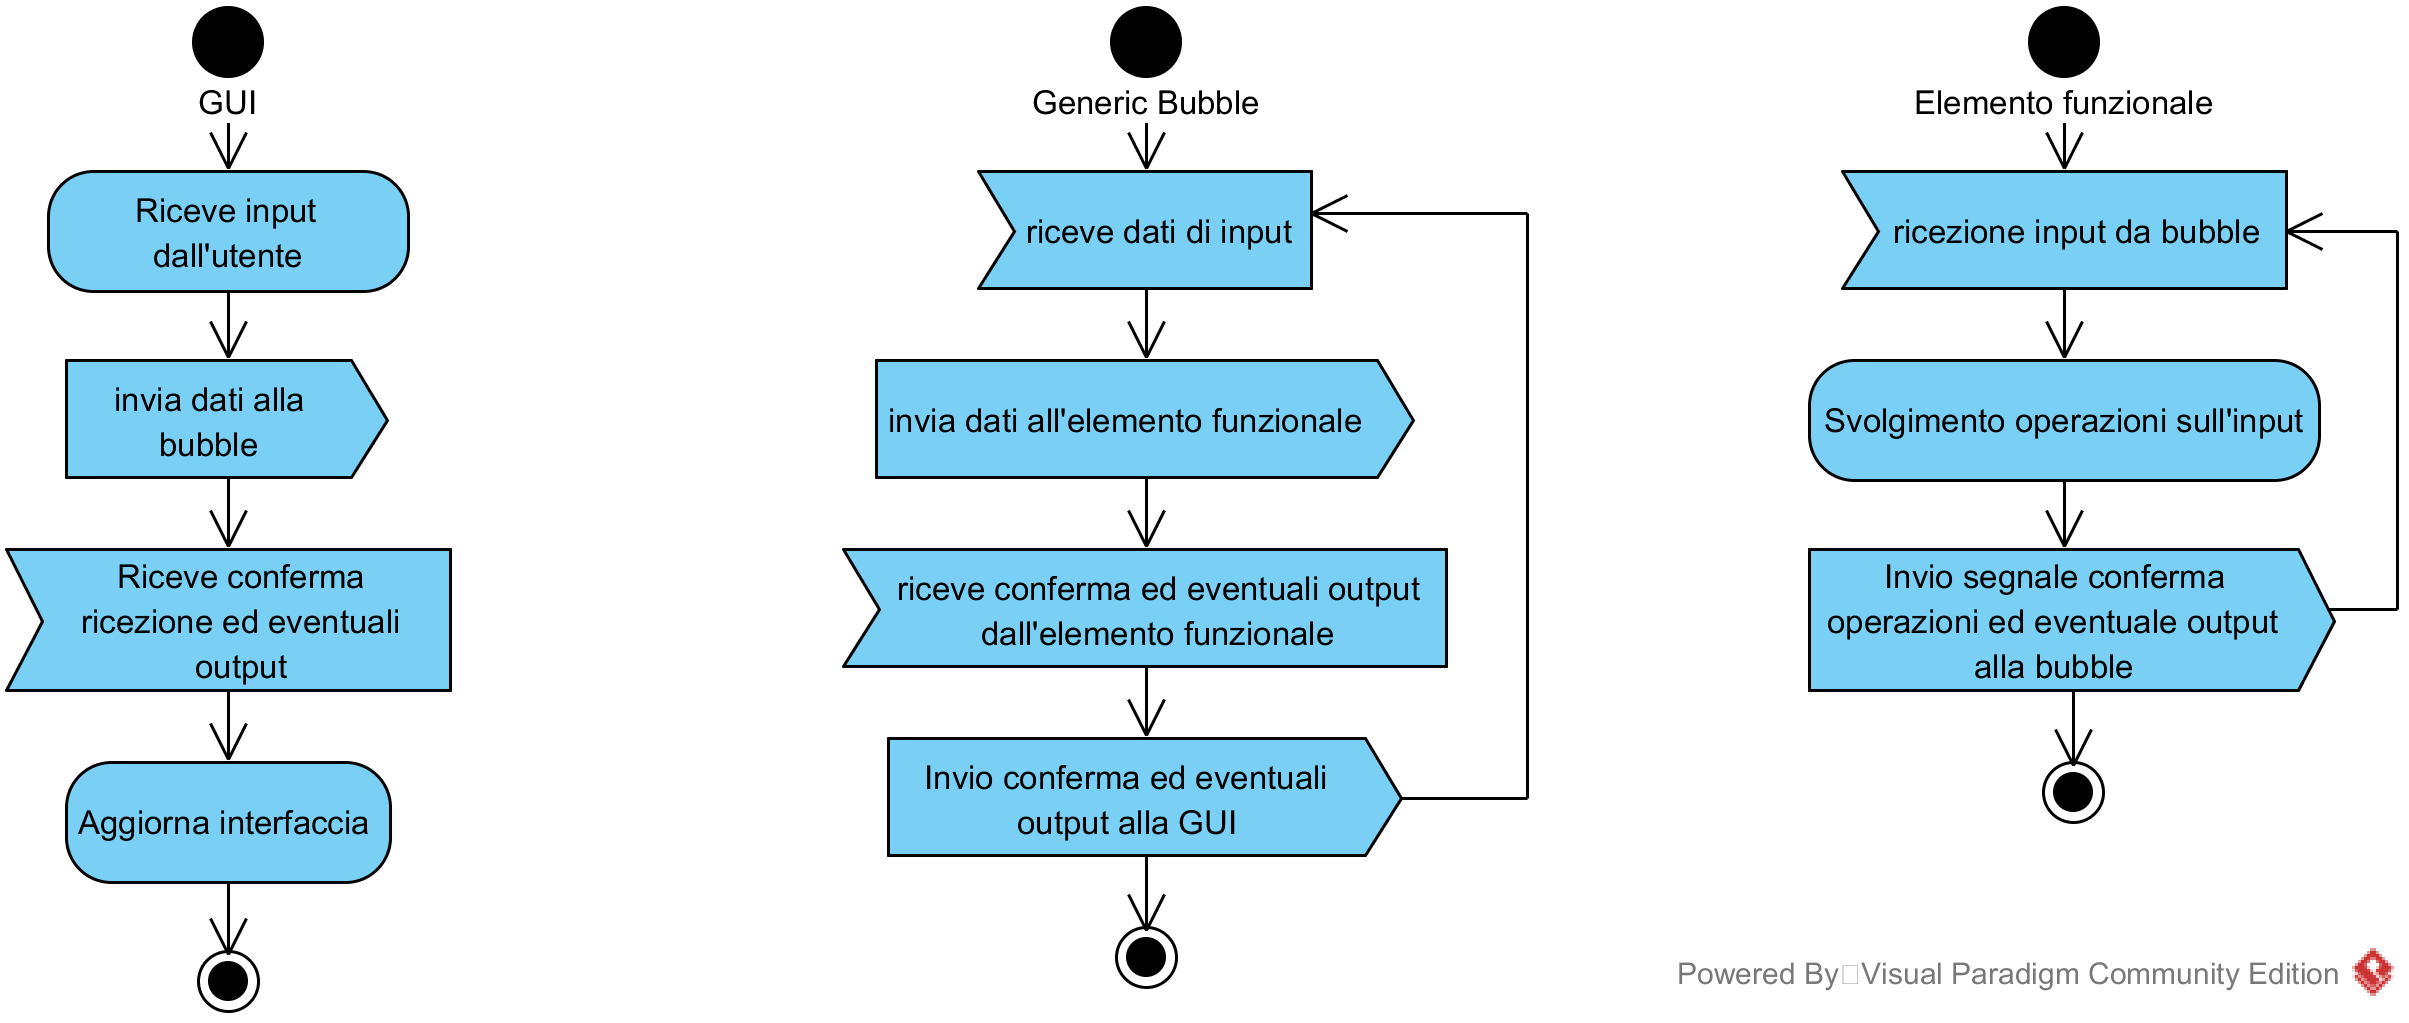
\includegraphics[width=14cm]{diagrammi_img/attivita/framework.png}
	\caption{Diagramma di attività - Framework}
	\label{fig:alt_framework}
\end{figure}
L'elemento della GUI riceve un input dall'utente e invia dei dati alla Generic Bubble, quindi rimane in attesa della conferma di ricezione ed eventuali output. La Generic Bubble, dopo aver ricevuto i dati, invia dei dati all'elemento funzionale e rimane anch'essa in attesa della conferma di ricezione ed eventuali output. L'elemento funzionale, una volta ricevuti i dati, svolge l'operazione richiesta e manda un segnale di risposta alla Generic bubble insieme all'eventuale output dell'operazione. La Generic bubble, una volta ricevuta la conferma, invia a sua volta un segnale di conferma e gli eventuali output alla GUI, la quale aggiorna l'interfaccia.

\begin{figure}[H]
	\centering
	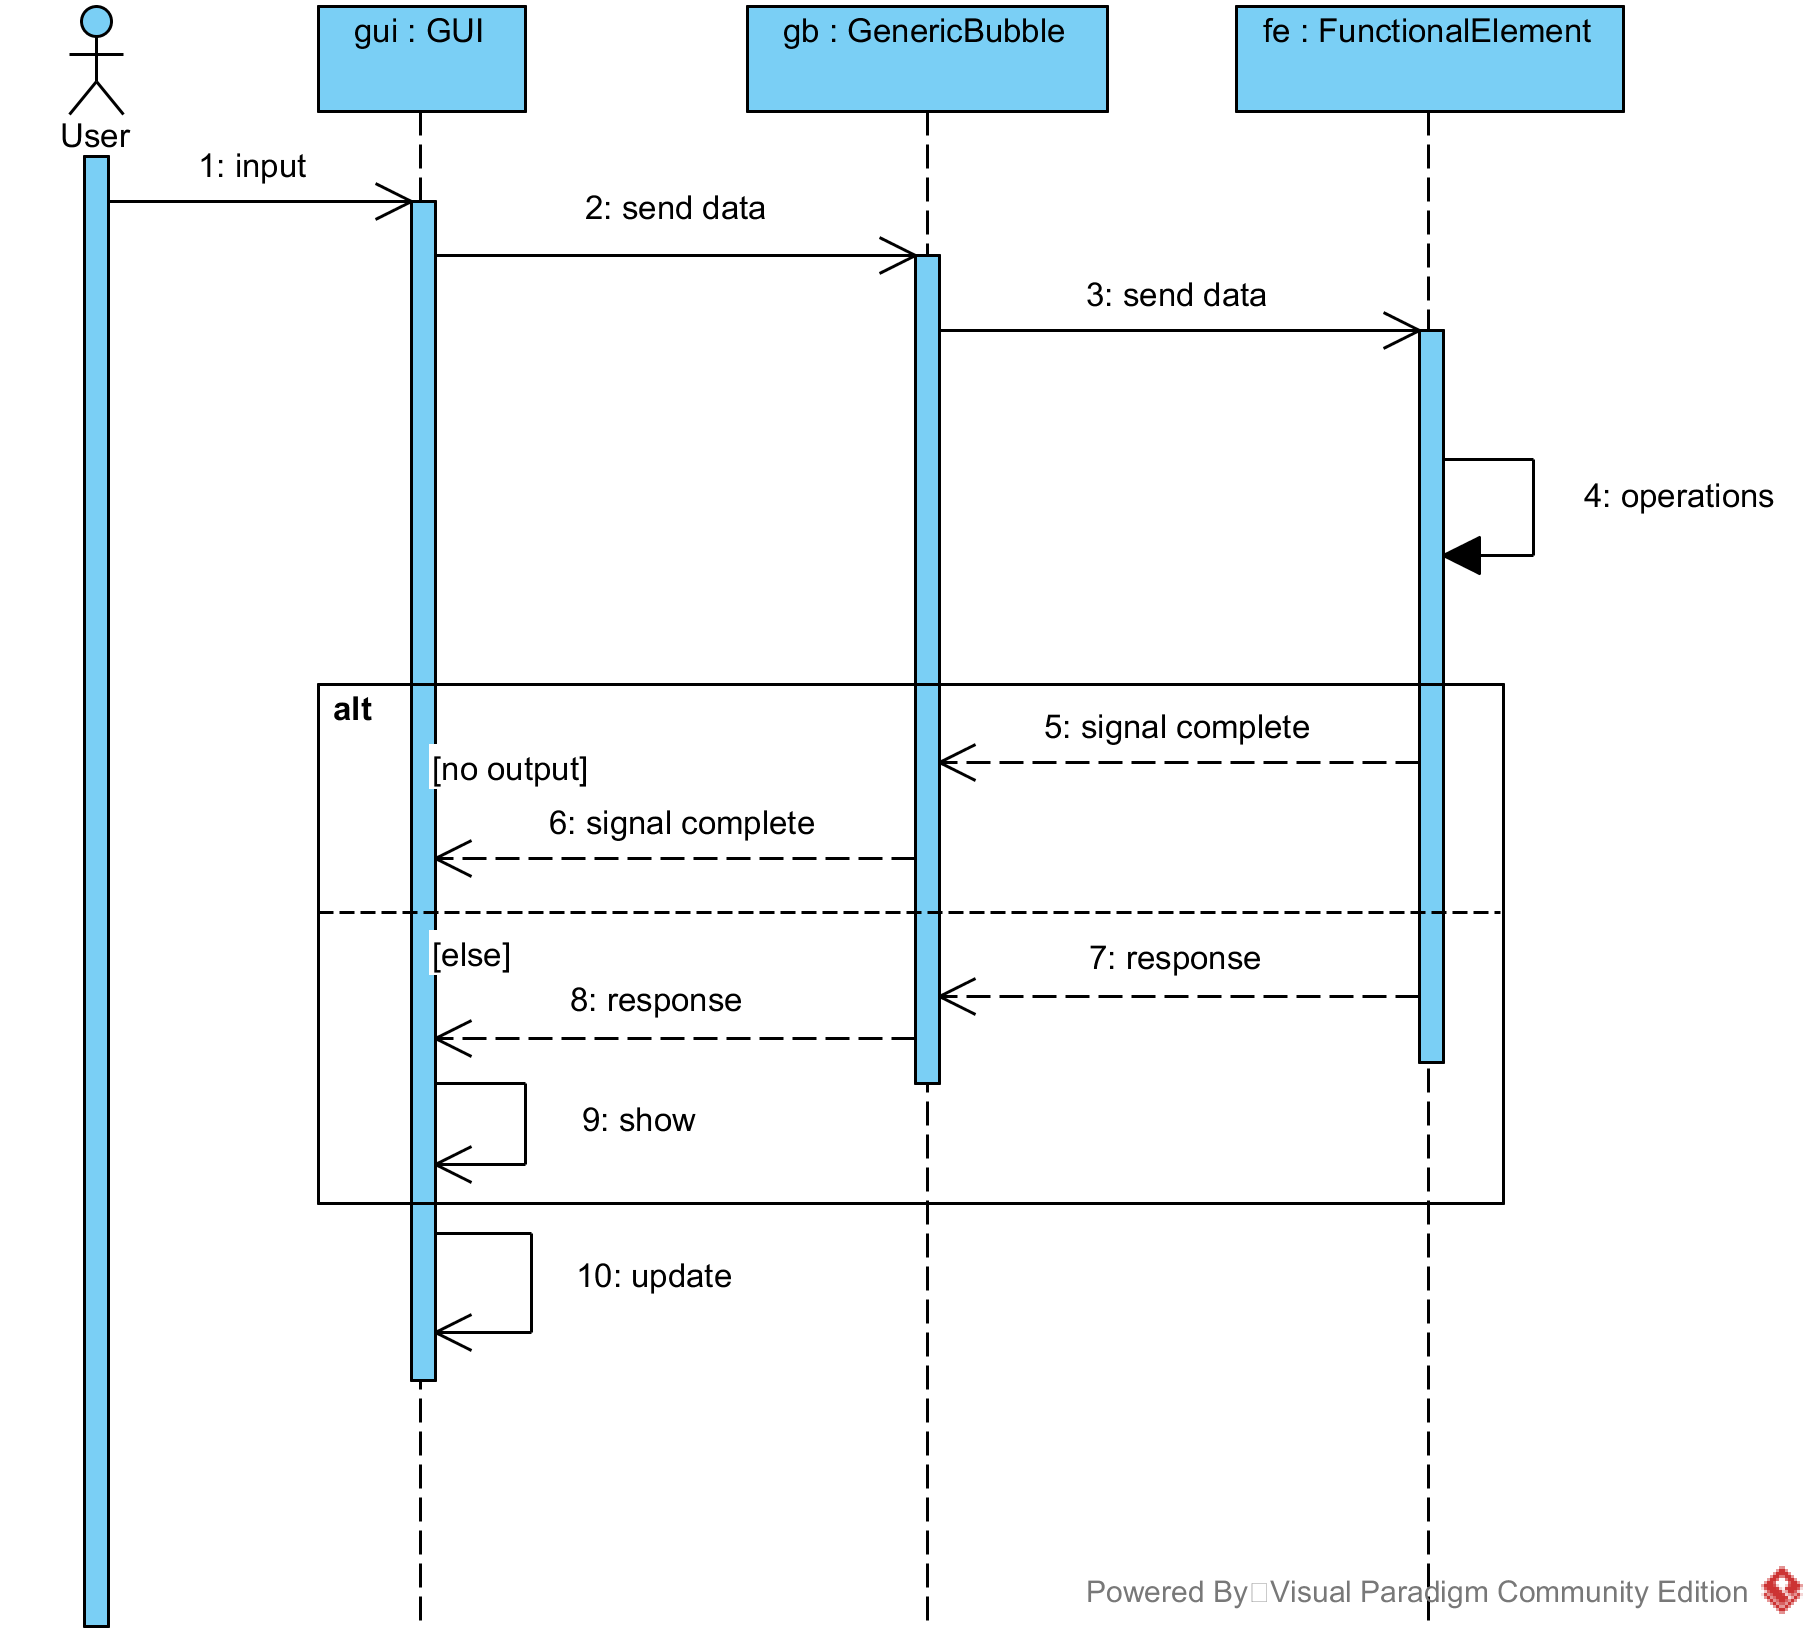
\includegraphics[width=14cm]{diagrammi_img/sequenza/framework.png}
	\caption{Diagramma di sequenza - Framework}
	\label{fig:seq_framework}
\end{figure}
Lo User da un input alla GUI, la quale invia dei dati alla GenericBubble. La GenericBubble invia anch'essa dei dati all FunctionalElement il quale svolge le operazioni richieste. Nel caso le operazioni non abbiano un output il FunctionalElement, dopo averle svolte, segnala il loro completamento alla GenericBubble che inoltra il segnale alla GUI. Nel caso in cui le operazioni abbiano un output FunctionalElement restituisce l'output alla GenericBubble che lo inoltra alla GUI, la quale mostra i risultati all'utente. In entrambi i casi al termine delle operazioni la GUI si aggiorna.
